\appendix{Представление графического материала}

Графический материал, выполненный на отдельных листах,
изображен на рисунках А.1--А.\arabic{числоПлакатов}.
\setcounter{числоПлакатов}{0}

\renewcommand{\thefigure}{А.\arabic{figure}} % шаблон номера для плакатов

\begin{landscape}
	
	\begin{плакат}
		
\includegraphics[width=0.82\linewidth]{Plakat1titlelist.eps}
		\заголовок{Сведения о ВКРБ}
		\label{pl1:image}      
	\end{плакат}
	
	\begin{плакат}
		
\includegraphics[width=0.82\linewidth]{zadachi.eps}
		\заголовок{Цели и задачи разработки}
		\label{pl2:image}      
	\end{плакат}
	
	\begin{плакат}
		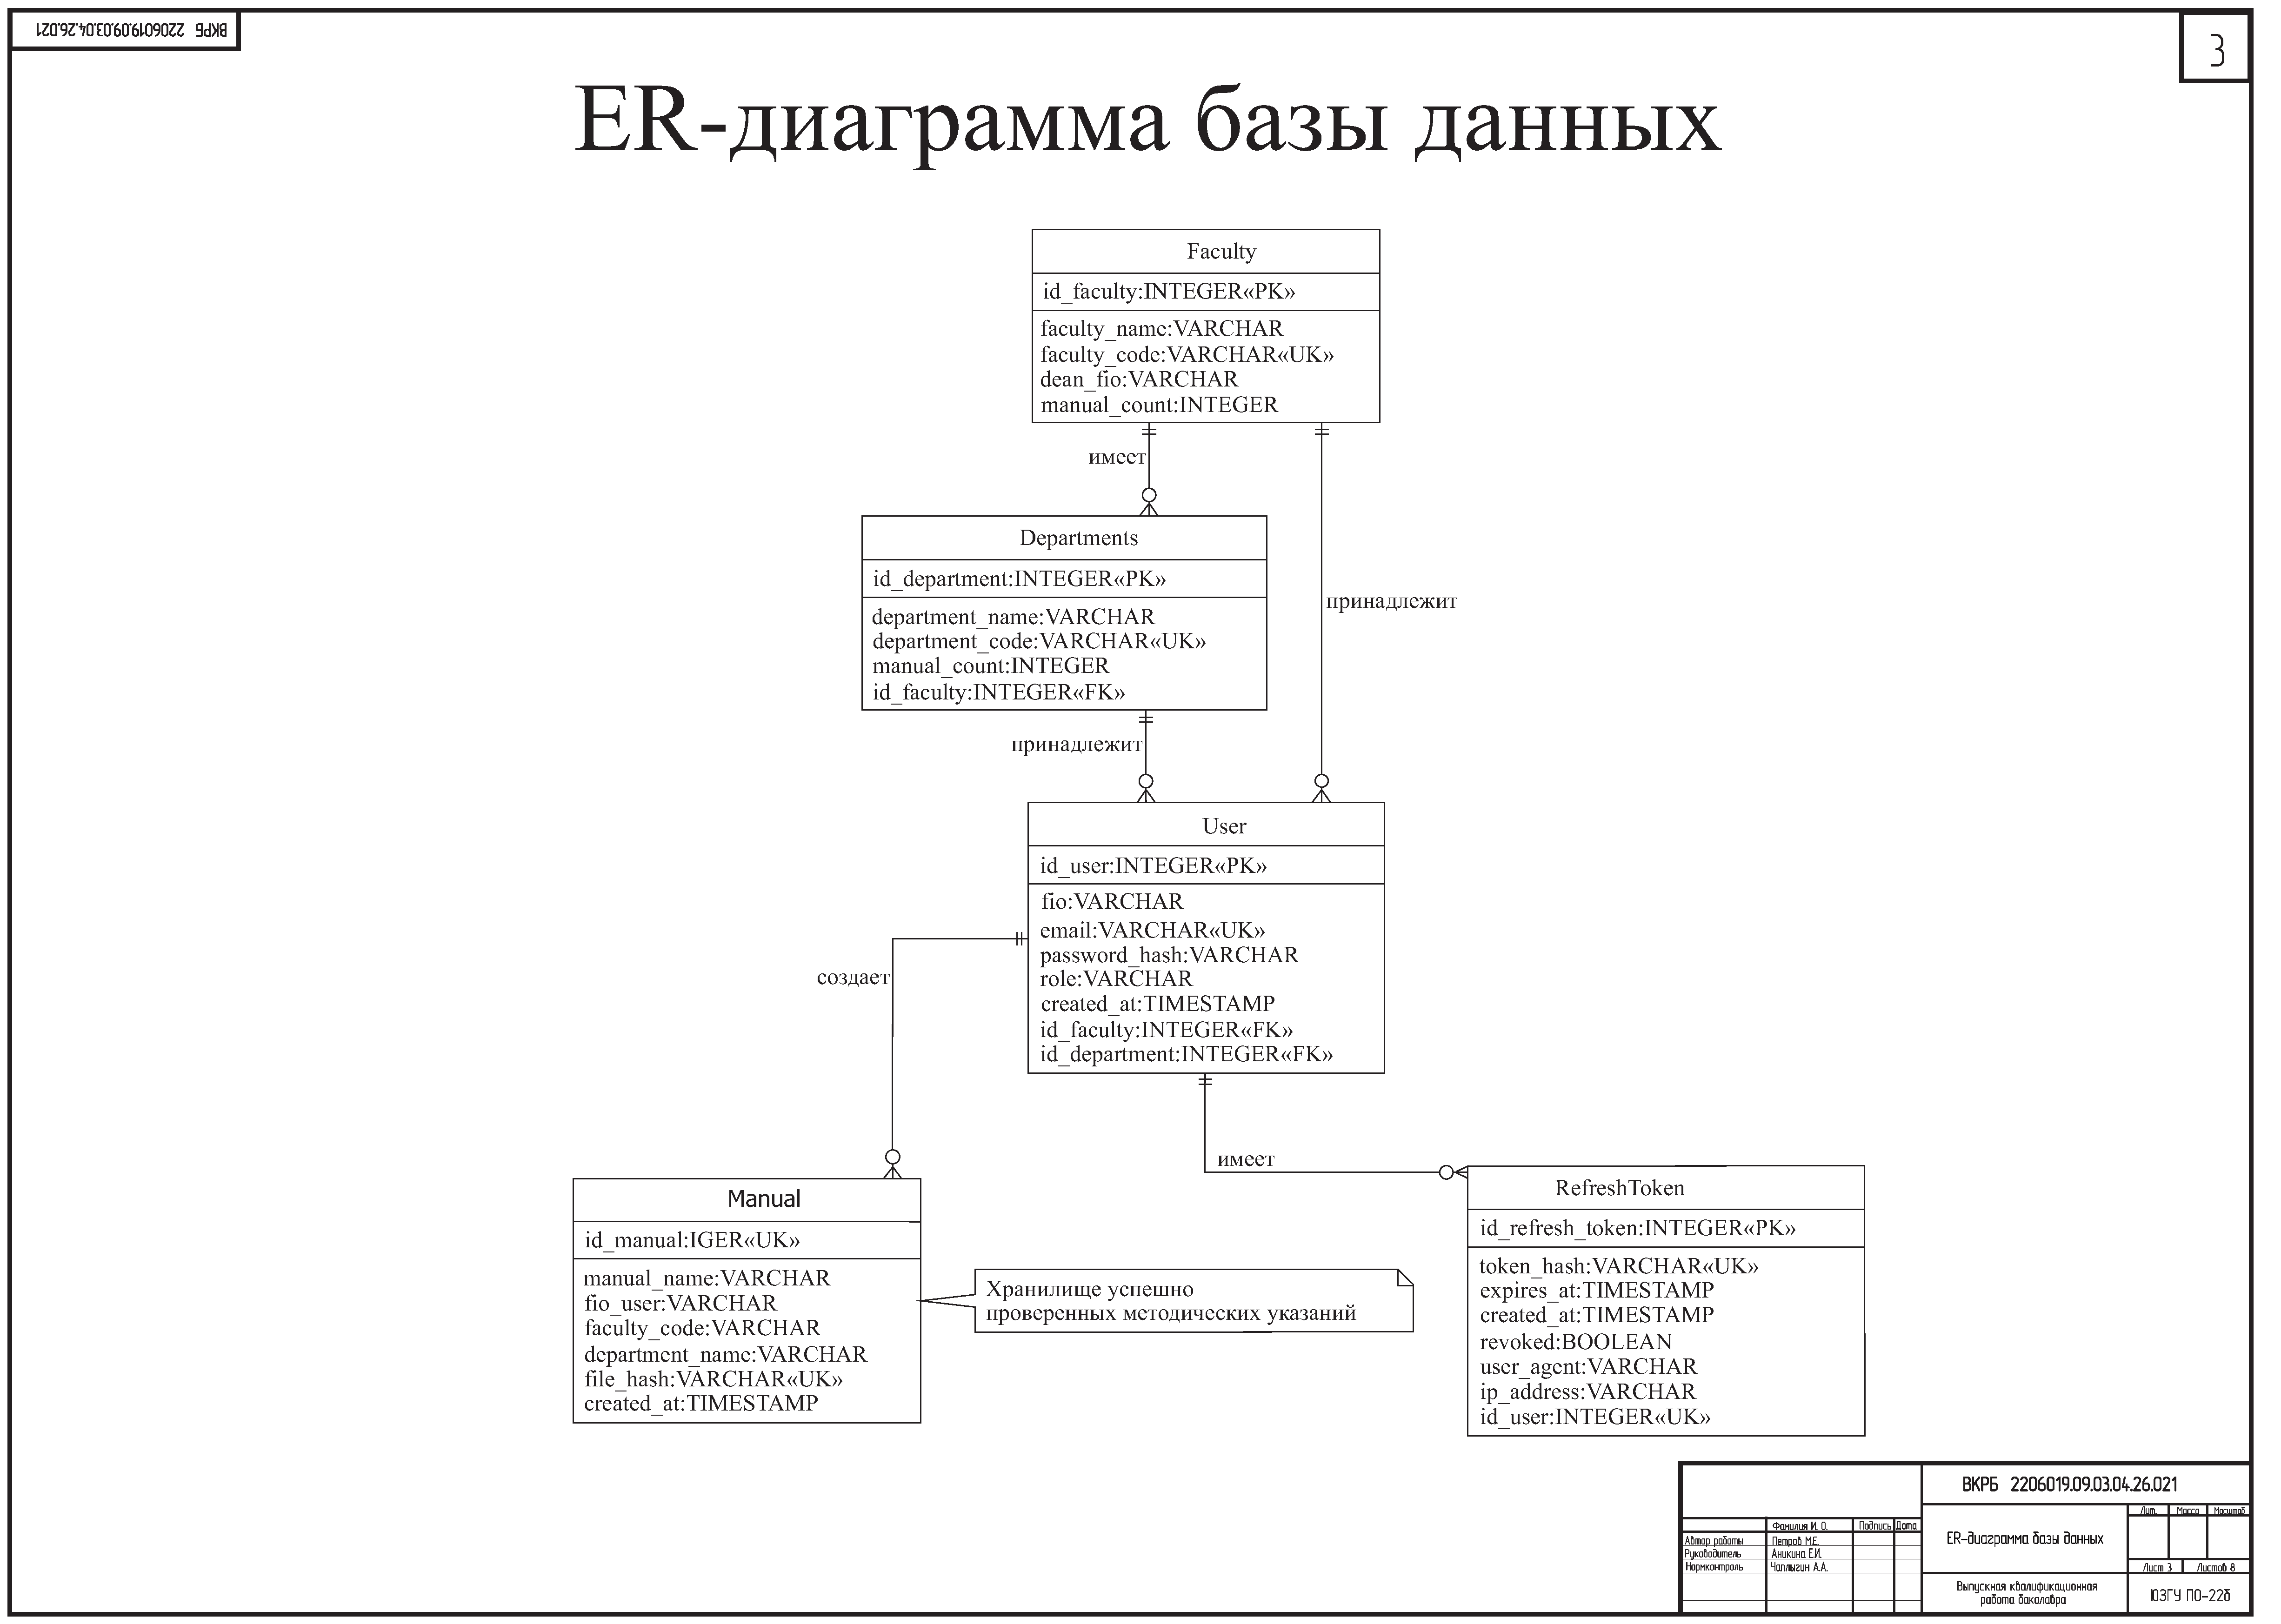
\includegraphics[width=0.82\linewidth]{Plakat2ERdiogramm.eps}
		\заголовок{ER-диаграмма базы данных}
		\label{pl3:image}      
	\end{плакат}
	
	\begin{плакат}
		
\includegraphics[width=0.82\linewidth]{Plakat3.eps}
		\заголовок{Реляционная модель базы данных}
		\label{pl4:image}      
	\end{плакат}
	
	\begin{плакат}
		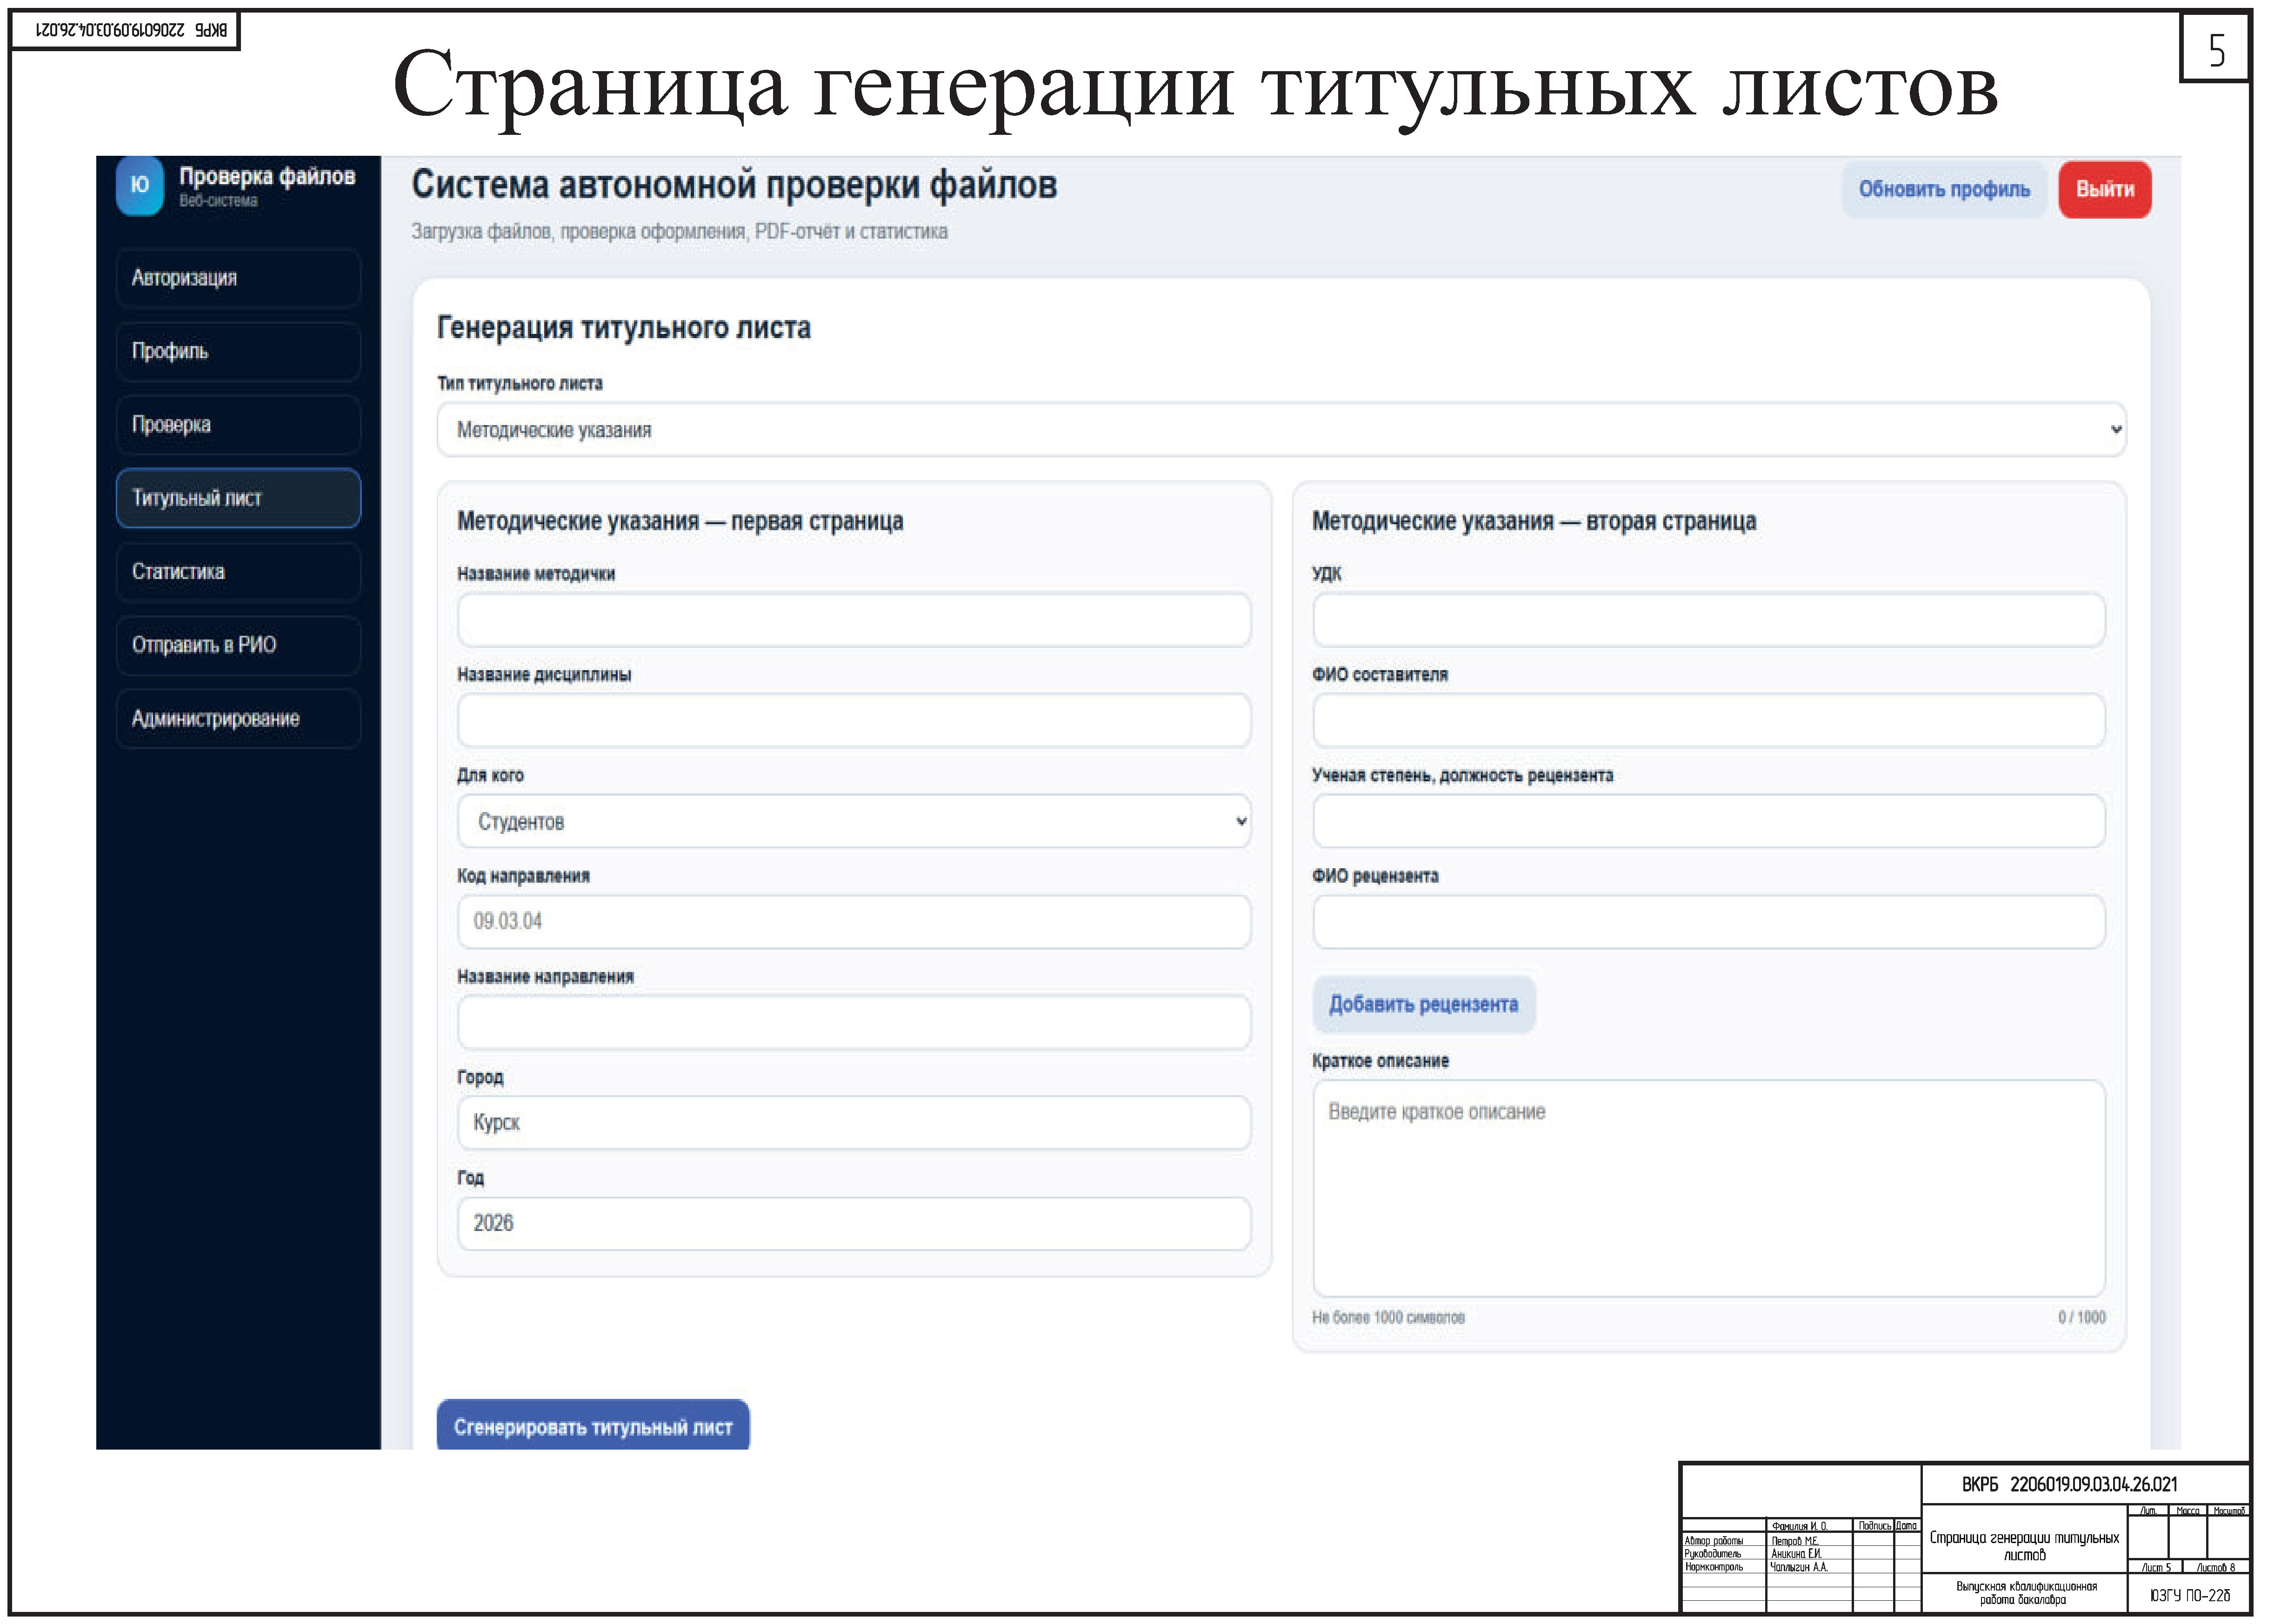
\includegraphics[width=0.82\linewidth]{Plakat5.eps}
		\заголовок{Страница генерации титульных листов}
		\label{pl5:image}      
	\end{плакат}
	
	\begin{плакат}
		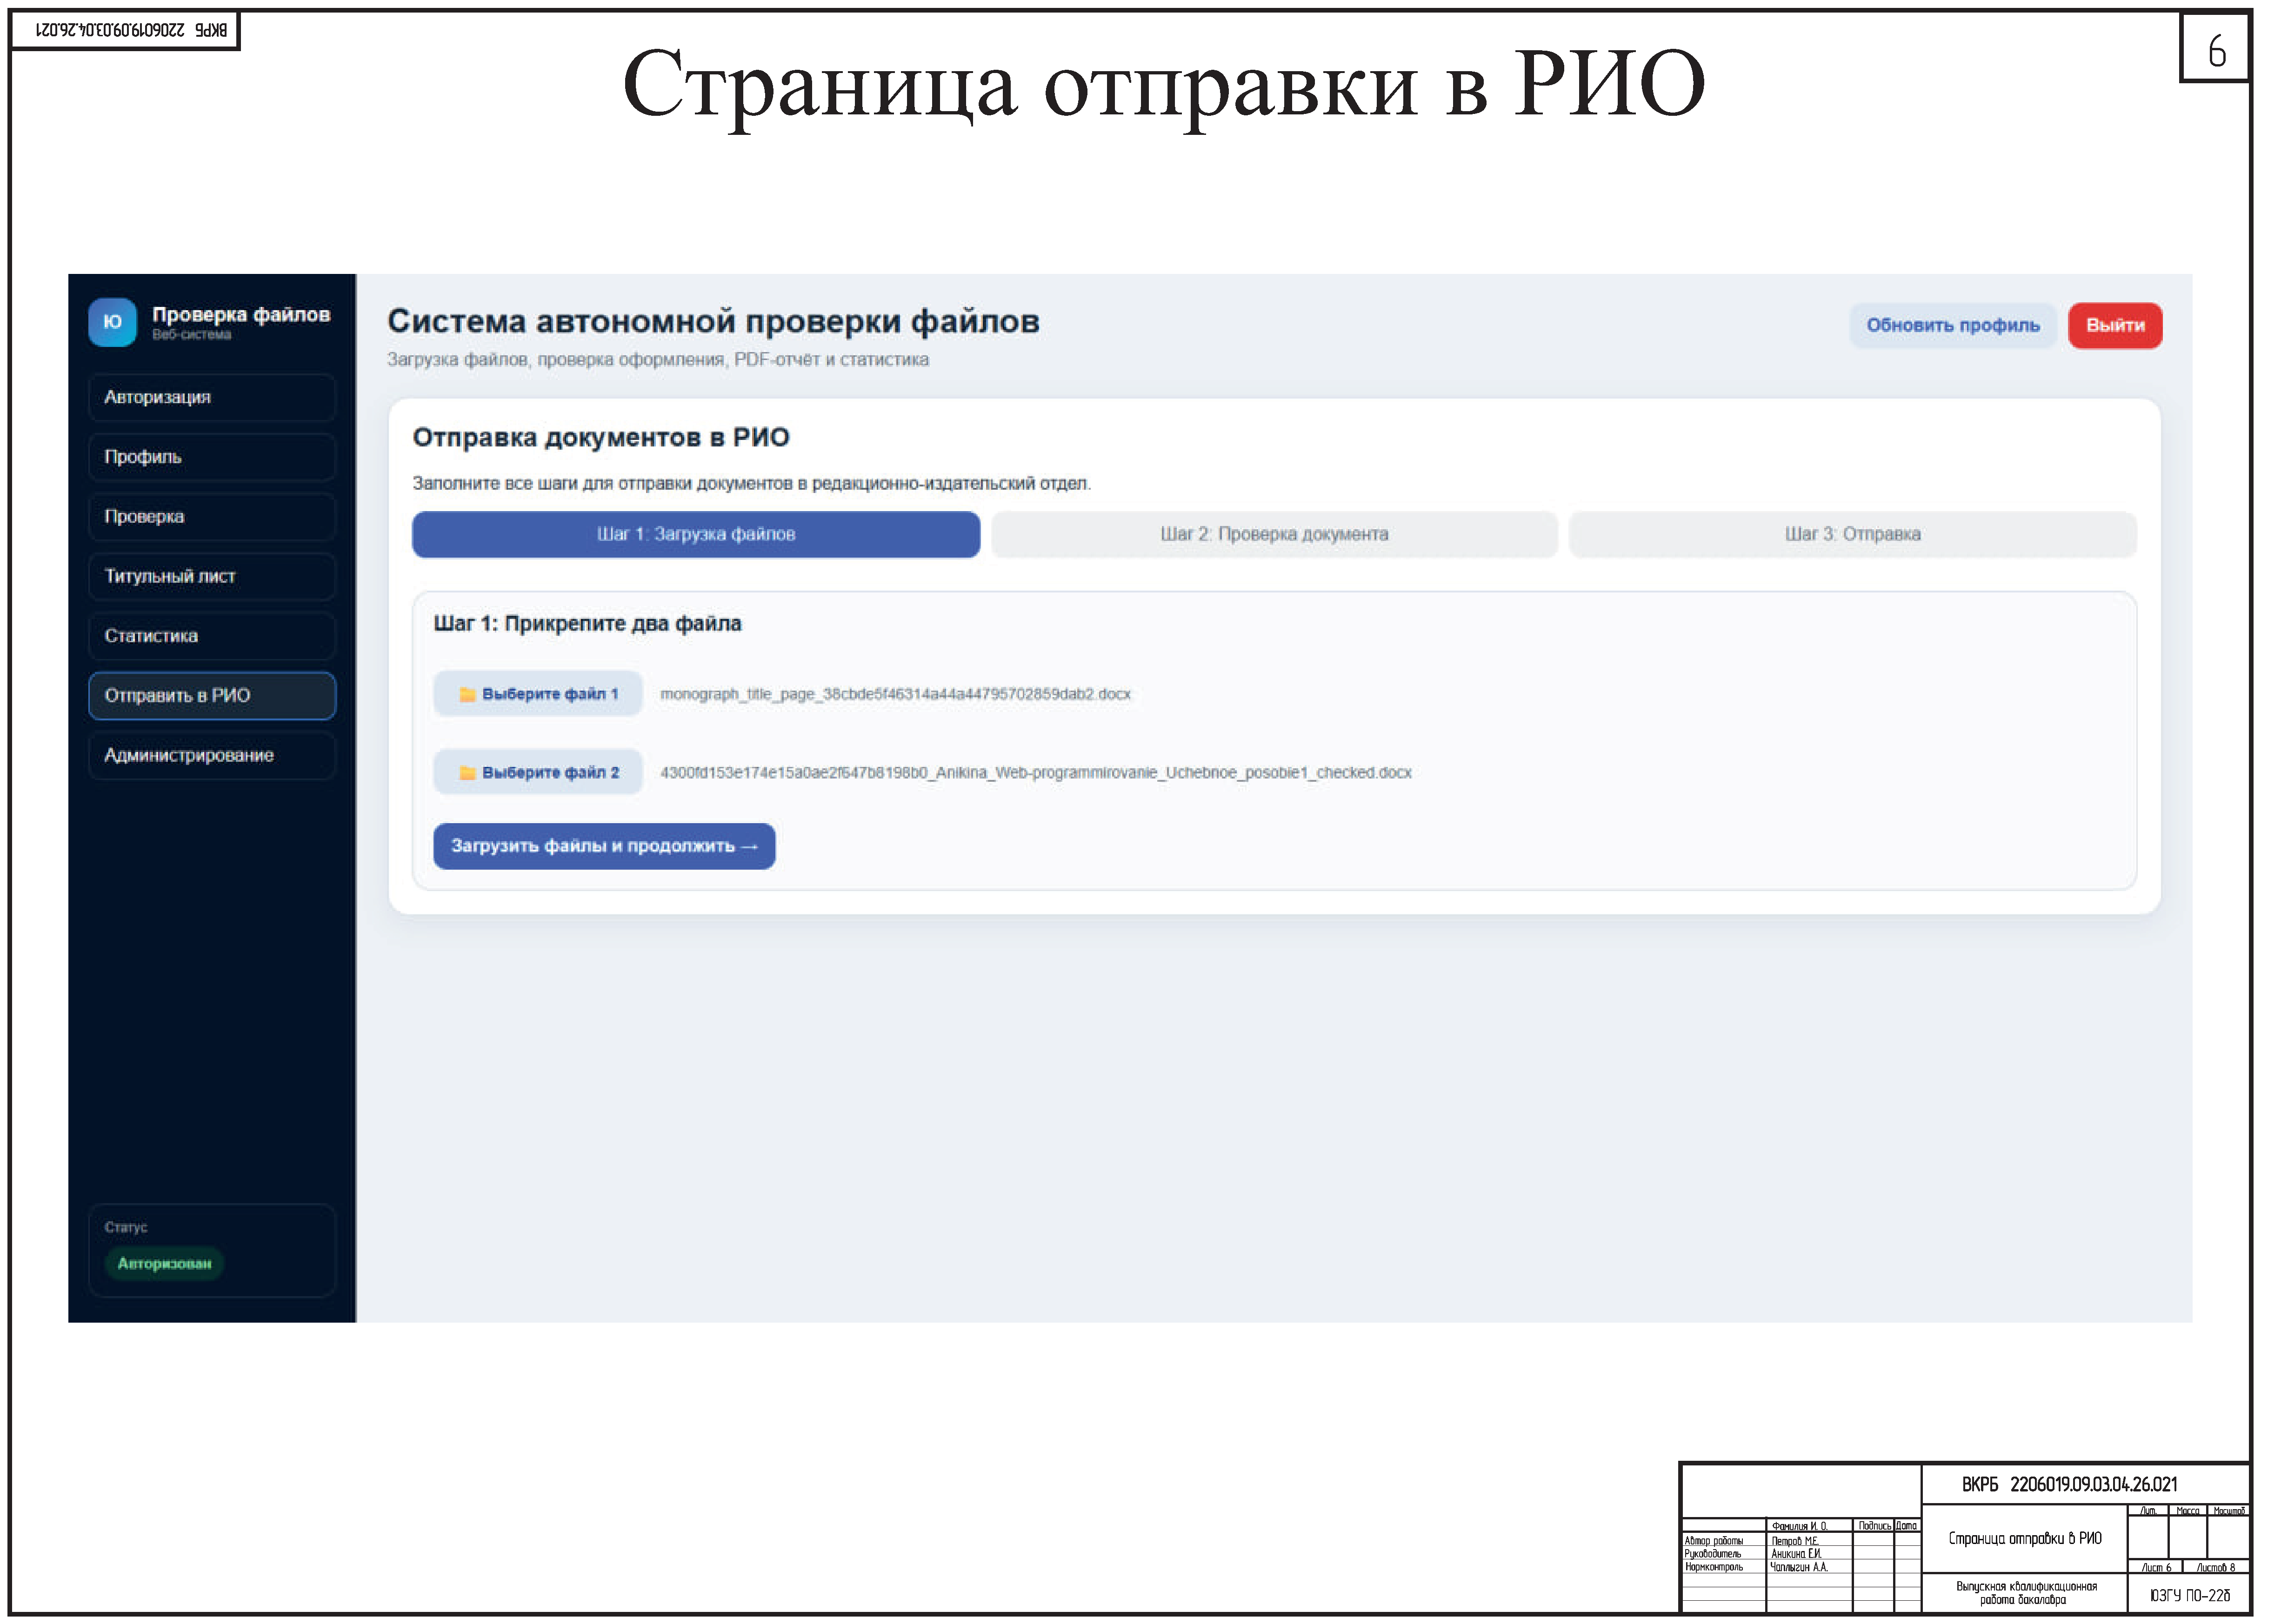
\includegraphics[width=0.82\linewidth]{Plakat6.eps}
		\заголовок{Страница отправки в РИО}
		\label{pl6:image}      
	\end{плакат}
	
	\begin{плакат}
		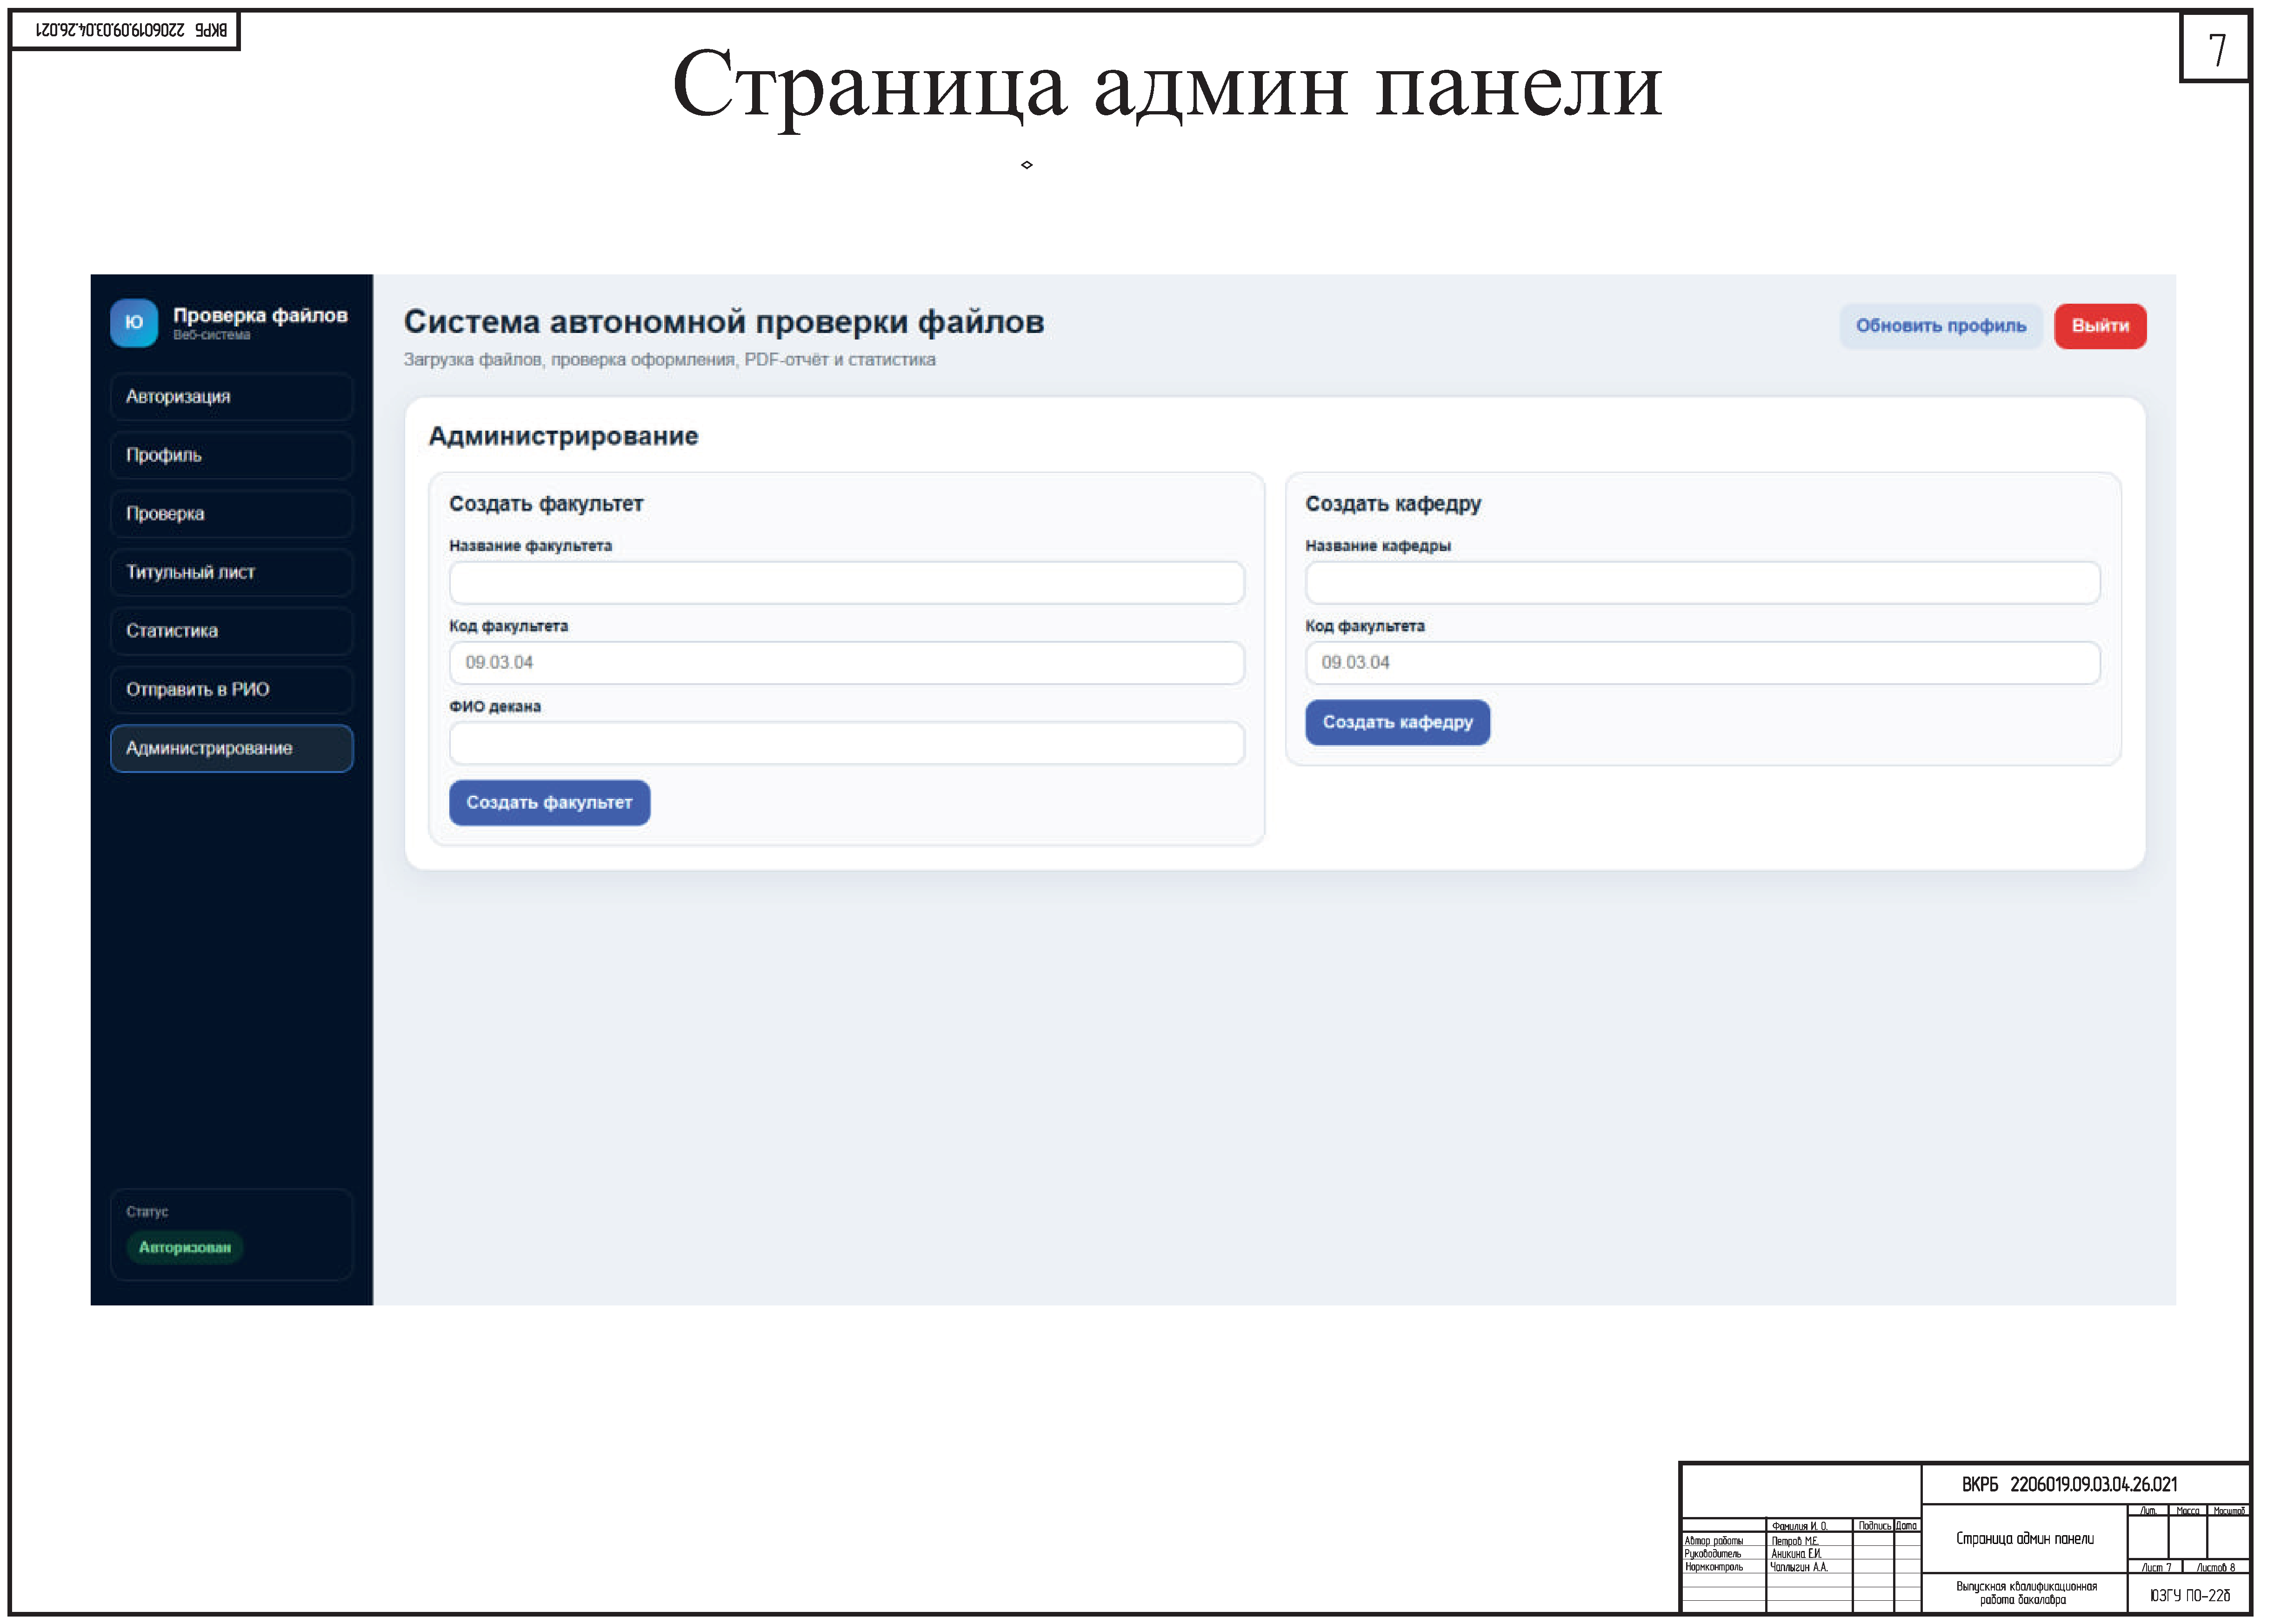
\includegraphics[width=0.82\linewidth]{Plakat7.eps}
		\заголовок{Страница админ панели}
		\label{pl7:image}      
	\end{плакат}
	
	\begin{плакат}
		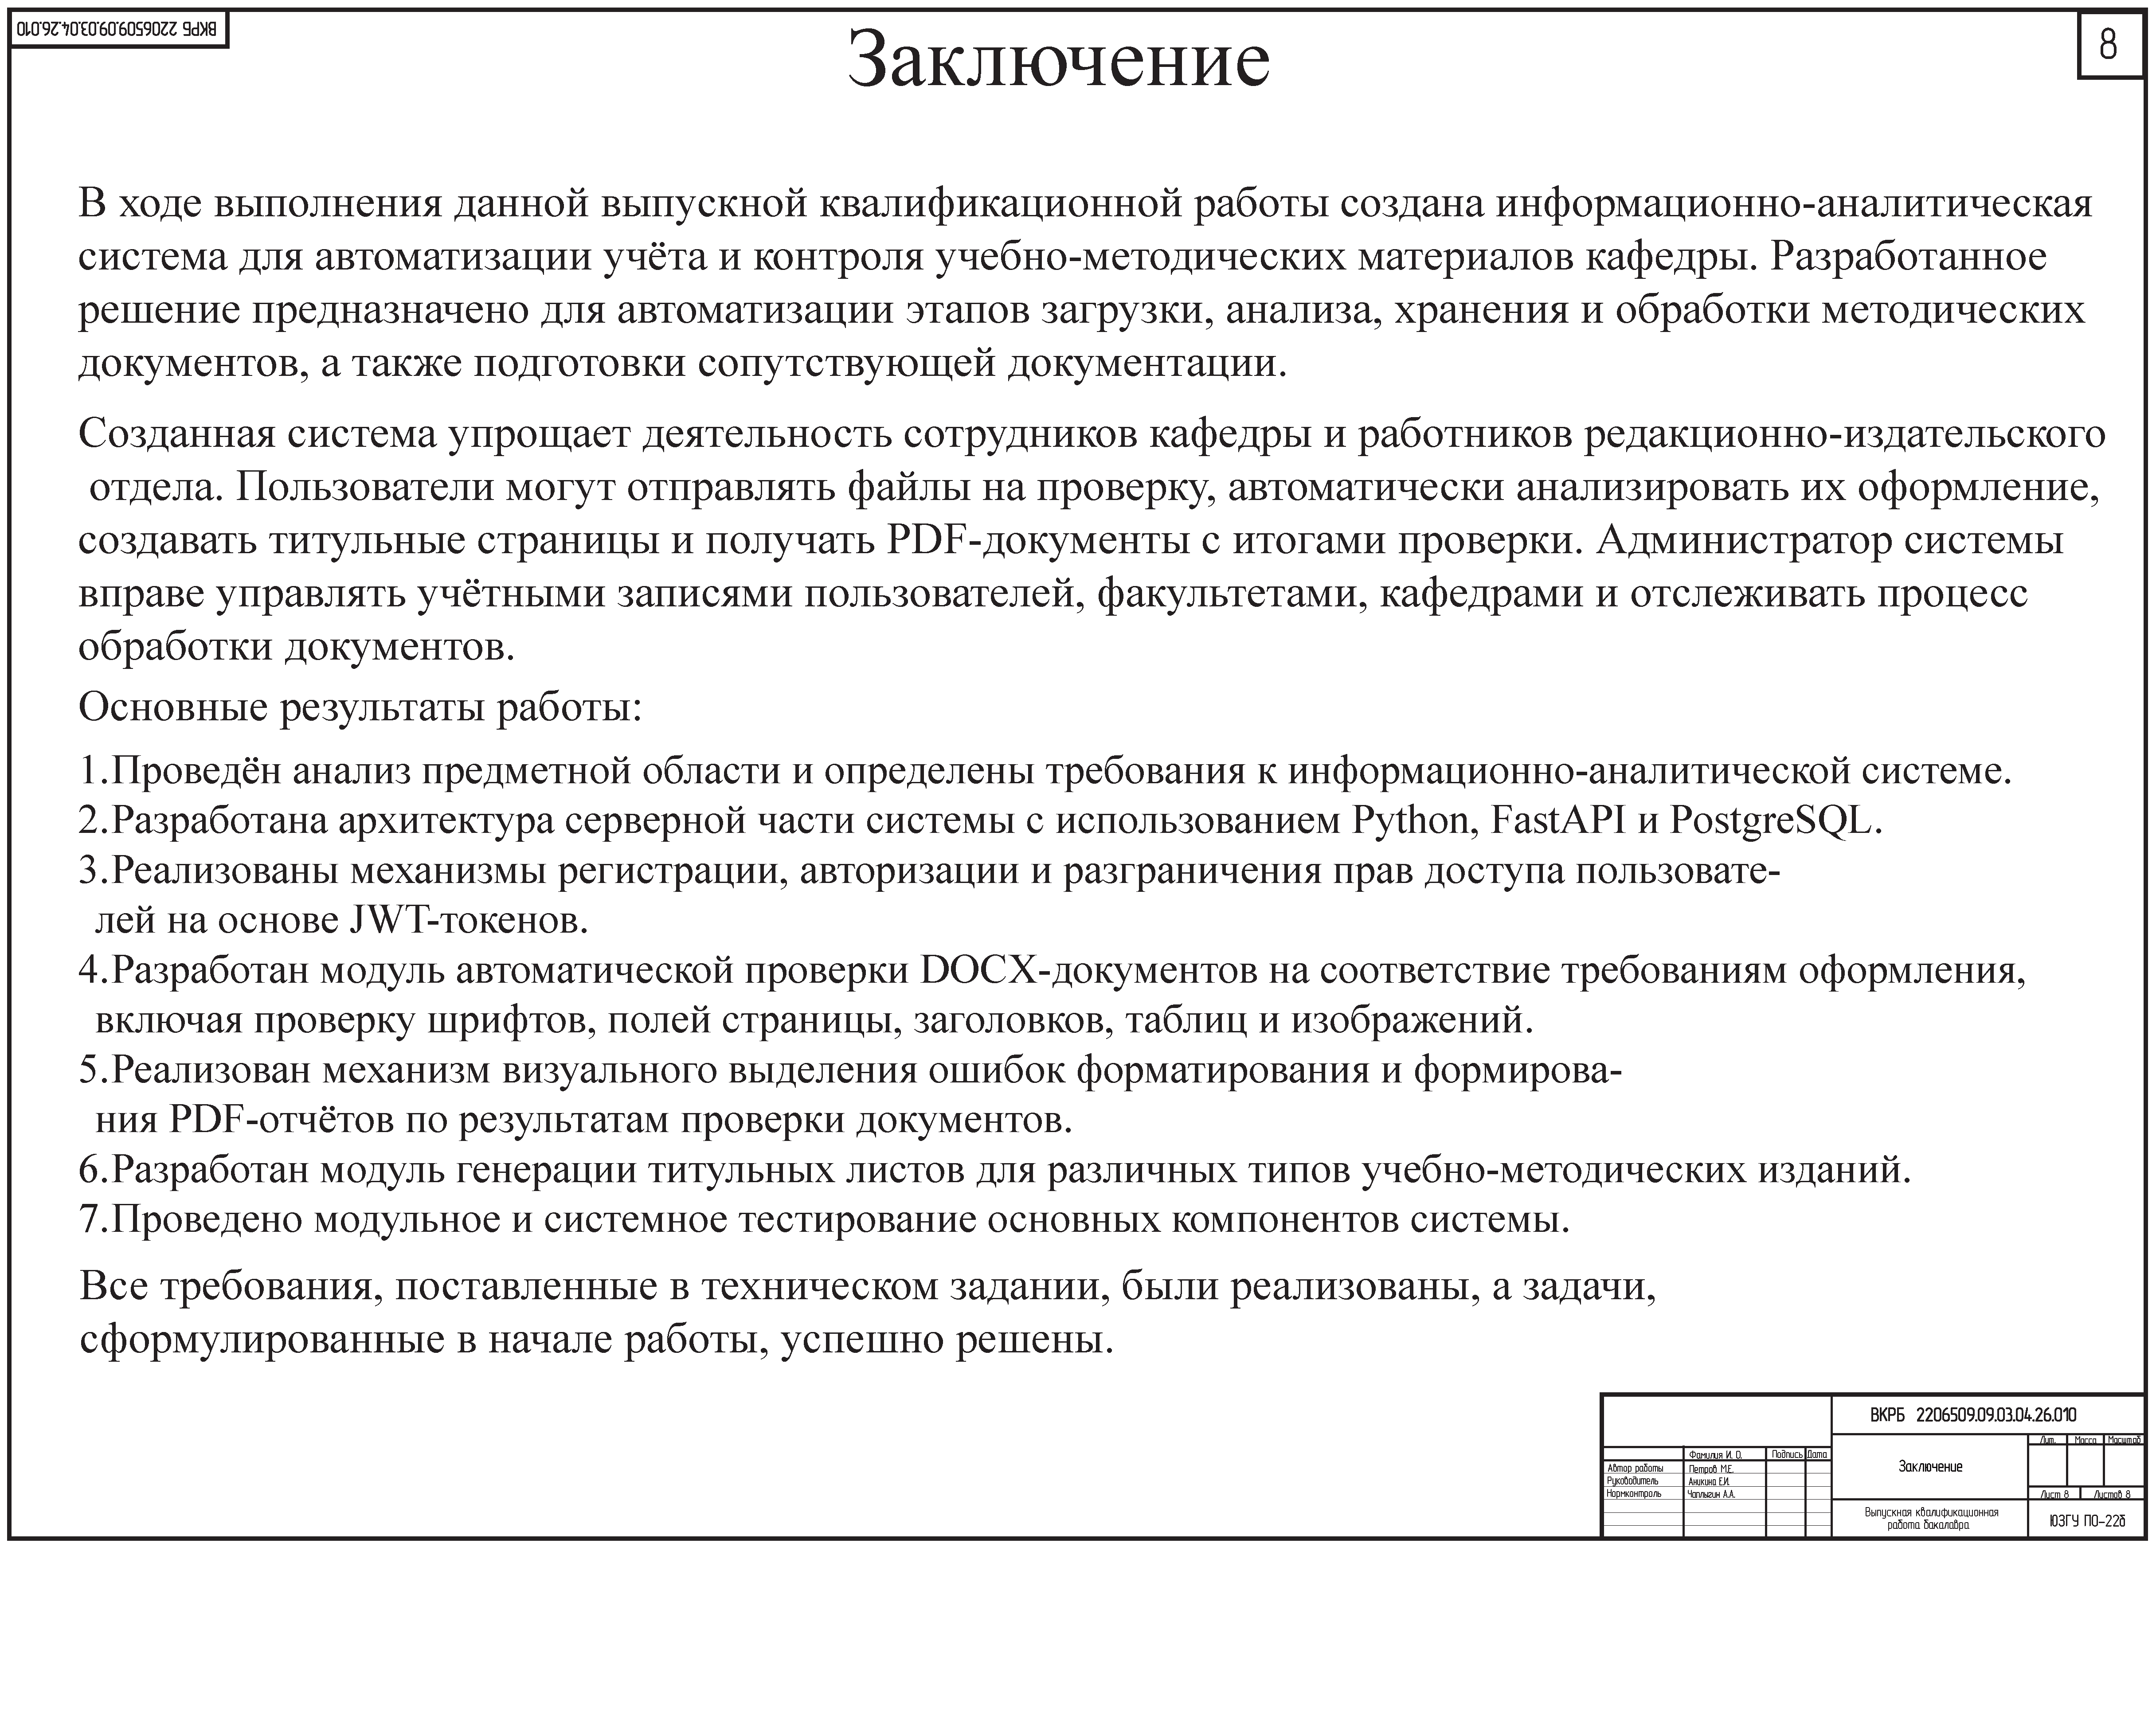
\includegraphics[width=0.82\linewidth]{Plakat8.eps}
		\заголовок{Заключение}
		\label{pl8:image}      
	\end{плакат}
	
\end{landscape}